\documentclass[11pt,a4paper]{jsarticle}

\input{include/macro.tex}
\input{include/preamble.tex}

\begin{document}

\section{ソフトウェア} \setcounters{0}

\subsection{アルゴリズム}
  機体周囲に放射状に取り付けられた測距センサによる距離情報をもとに障害物回避を行う.

  まず,スカラーである距離情報に方向の情報を付加するために,
  実際の機体周囲の測距センサの配置を元に,
  次のように8つの二次元単位ベクトルを定義する.

  \begin{eqnarray}
    \bm{u}_0 = \begin{bmatrix} -0.707 \\ -0.707 \end{bmatrix}, \hspace{5mm} \nonumber
    \bm{u}_1 = \begin{bmatrix}  0     \\ -1     \end{bmatrix}, \hspace{5mm}
    \bm{u}_2 = \begin{bmatrix}  0.707 \\ -0.707 \end{bmatrix}, \hspace{5mm}
    \bm{u}_3 = \begin{bmatrix}  1     \\  0     \end{bmatrix}, \hspace{5mm} \\[3mm]
    \bm{u}_4 = \begin{bmatrix}  0.707 \\  0.707 \end{bmatrix}, \hspace{5mm} \nonumber
    \bm{u}_5 = \begin{bmatrix}  0     \\  1     \end{bmatrix}, \hspace{5mm}
    \bm{u}_6 = \begin{bmatrix} -0.707 \\  0707  \end{bmatrix}, \hspace{5mm}
    \bm{u}_7 = \begin{bmatrix} -1     \\  0     \end{bmatrix}  \hspace{5mm} \\ \nonumber
  \end{eqnarray}

  距離センサのセンサ値$v$より距離$d \unit{cm}$を求める式は次の2式である.

  \begin{eqnarray}
    d_{\rm{ long}} &=& 45.514 v^{-0.822} \\
    d_{\rm{short}} &=& 0.09999 v + 0.4477 \\ \nonumber
  \end{eqnarray}

  障害物との衝突を避けるため,センサにより得られた距離が小さいほど大きな斥力が
  機体の進行方向に作用するようにしなければならない.
  また同時に,離れすぎることも競技エリア外に出てしまうことが懸念されるため避けなければならない.
  そのため,距離が大きい時には大きな負の斥力,すなわち障害物からの引力を受けるように,
  次の式を利用して距離情報を『危険度』の情報に変換する.

  \begin{equation}
    y = -\tanh^{-1}(x-1) \label{eq::arctanh}
  \end{equation}

  \refeq{arctanh}を図に表すと\refig{arctanh}となる.

  \begin{figure}[b]
    \begin{center}
      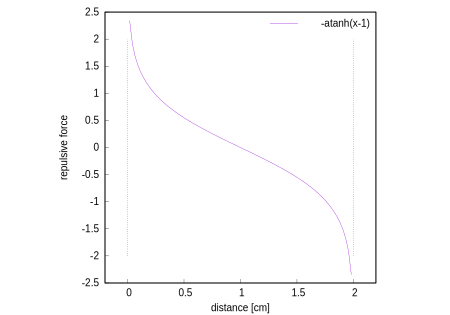
\includegraphics[width=1.0\hsize]{plot/minus_atanh.eps}
    \end{center}
    \caption{$y=-\tanh^{-1}(x-1)$}
    \label{fig::arctanh}
  \end{figure}

  実際には適正距離で$\tanh^{-1}(x-1) = 0$となるように,
  維持したい距離とセンサの最大レンジないしは採用する最大の距離を考慮に入れて,
  それらを正規化した値を代入しなければならない.

  また,零距離から適正距離,適正距離から最大距離の比が$1:1$とならない場合は,
  場合を分けて正規化を行わなければならない.\\

\subsection{画像認識}
  炎上ポールの認識には配布されたRapspberry Pi NoIR Camera V2(以下,カメラモジュール)を使用する.
  画像撮影から最も近いポールと思われる物体へのベクトルを出力する一連の手順を,簡単に以下に示す.
  画像処理にはOpenCVライブラリを用いており,各処理で使用した主要なライブラリ関数を併記する.

  \begin{description}

    \item[画像取得] \mbox{} \\
      カメラモジュールへのアクセスには既成ライブラリ\cite{raspicam}を利用した.
      撮影によりピクセル値の2次元配列(cv::Mat)が出力として得られる.\\

    \item[カラーモデル変換] \mbox{} \\
      得られた画像のカラーモデルをRGBからHSVに変更する.\\
      使用関数:\texttt{cv::cvtColor} \\

    \item[2値画像化] \mbox{} \\
      HSV画像データに対し赤色マスクをかけて2値画像に変換する.\\
      使用関数:\texttt{cv::inRange} \\

    \item[ノイズ除去] \mbox{} \\
      モルフォロジー処理によりノイズを除去する.\\
      使用関数:\texttt{cv::morphologyEx} \\

    \item[構造解析] \mbox{} \\
      2値画像中の輪郭線を検出した後,それを矩形で囲む.
      囲んだ矩形を縦横比で解析し,ポールの縦横比に対して$\pm 20 \%$以上の差があるものを除外する.\\
      使用関数:\texttt{cv::findContours},\texttt{cv::boundingRect} \\

    \item[ベクトル作成] \mbox{} \\
      除外されず残った矩形の重心点を求め,カメラの画角($62.2 \times 48.8$ \cite{elinux})
      を元に機体中心から重心点へ向かうベクトルを作る.\\
      使用関数:\texttt{cv::moments} \\

  \end{description}

\begin{thebibliography}{9}
  \bibitem{raspicam}
    "RaspiCam: C++ API for using Raspberry camera with/without OpenCV",\\
    "\texttt{https://www.uco.es/investiga/grupos/ava/node/40}",\\
    2017年5月31日最終確認.
  \bibitem{elinux}
    "RPi Camera Module - eLinux.org",\\
    "\texttt{http://elinux.org/Rpi\_Camera\_Module\#Technical\_Parameters\_.28v.2\_board.29}",\\
    2017年5月31日最終確認.
\end{thebibliography}

\end{document}
